\setAuthor{Ardi Loot}
\setRound{lõppvoor}
\setYear{2018}
\setNumber{G 5}
\setDifficulty{7}
\setTopic{Termodünaamika}

\prob{Soojustus}
\begin{wrapfigure}[10]{r}{0.5\textwidth}
\vspace{-30pt}
\begin{center}
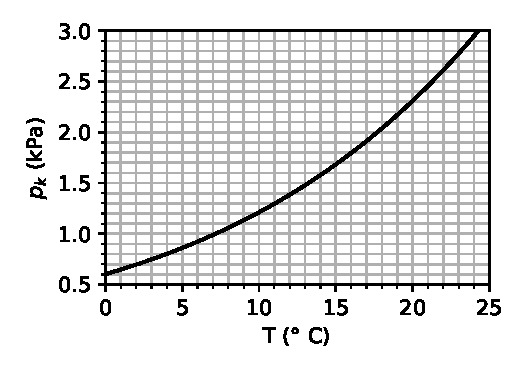
\includegraphics[width=0.5\textwidth]{2018-v3g-05-kullastunud-aur}
\par\end{center} 
\end{wrapfigure}

Seina soojustus koosneb sisemisest (soojusjuhtivus $k_{1}=\SI{0.07}{W/\left(m\cdot K\right)}$)
ja välimisest kihist (soojusjuhtivus $k_{2}=\SI{0.05}{W/\left(m\cdot K\right)}$).
Nende kihtide vahel on kile, et takistada õhu liikumist läbi seina.
Millist tingimust peab rahuldama sisemise soojustuskihi pakus $L_{1},$
et vältida veeauru kondenseerumist seinas? Seina paksus $L=L_{1}+L_{2}=\SI{30}{cm},$
$L_{2}$ on välimise soojustuskihi paksus, toa temperatuur $T_{1}=\SI{20}{\degreeCelsius},$
suhteline õhuniiskus toas $\eta_{1}=\SI{60}{\percent}$ ja välistemperatuur
$T_{2}=\SI{-20}{\degreeCelsius}.$ Küllastunud veeauru osarõhu sõltuvus
temperatuurist on toodud joonisel.

\emph{Märkus.} Eeldada, et temperatuur muutub soojustuskihis lineaarselt
kaugusega ja muutuse kiirus on pöördvõrdeline soojusjuhtivusega. 

\hint
Selleks, soojustuskihtide vahel oleval kilel vältida kondenseerumist, ei tohi kile asukohas temperatuur
langeda alla kastepunkti. Kastepunkt on leitav graafikult, leides veeauru osarõhu toatemperatuuril ning seejärel leides sellele vastava kastepunkti.

\solu
Toas oleva niiske õhu levikut piirab soojustuskihtide vahel olev kile.
Selleks, et vältida kondenseerumist, ei tohi kile asukohas temperatuur
langeda alla kastepunkti. 

Kastepunkti saame leida graafiku alusel, leides alguses küllastunud
veeauru osarõhu toatemperatuuril, arvutades sellest $\eta_{1}=\SI{60}{\percent}$
ja seejärel leides sellele vastava kastepunkti $T_{k}=\SI{12.0}{\degreeCelsius}.$
\begin{center}
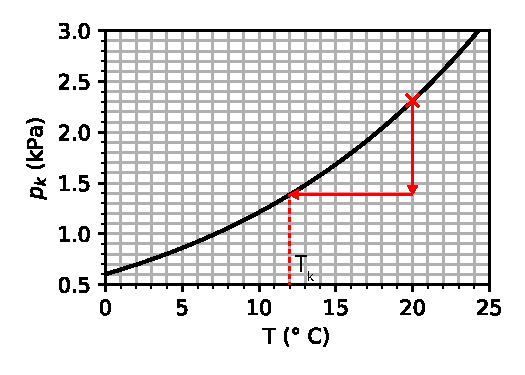
\includegraphics[scale=0.9]{2018-v3g-05-kullastunud-aur-lah}
\par\end{center}

Järgmiseks on vaja leida avaldis temperatuuri jaoks kile asukohas
($T$). Eeldades, et temperatuur muutub soojustuskihis lineaarselt
kaugusega ja muutuse kiirus on pöördvõrdeline soojusjuhtivusega, saame
liikudes seest välja kirja panna kaks võrrandit:

\begin{equation*}
\begin{cases}
\begin{array}{c}
T=T_{1}-\frac{\alpha}{k_{1}}L_{1}\\
T_{2}=T-\frac{\alpha}{k_{2}}L_{2},
\end{array}
\end{cases}
\end{equation*}

\noindent kus $\alpha$ on tundmatu võrdetegur. Nende võrrandite lahendamine
annab

\begin{equation*}
T=\frac{k_{2}T_{2}L_{1}+k_{1}T_{1}L_{2}}{k_{2}L_{1}+k_{1}L_{2}}.
\end{equation*}

Ja lõpetuseks, tuleb leida sisemise soojustuskihi paksus $L_{1}$
piirjuhul, kui kile temperatuur võrdub kastepunktiga

\begin{equation*}
L_{1}=L\frac{k_{1}\left(T_{1}-T_{k}\right)}{k_{1}T_{1}-k_{2}T_{2}-\left(k_{1}-k_{2}\right)T_{k}}\approx\SI{7.8}{cm}
\end{equation*}

\noindent ja kondenseerumise vältimiseks peab sisemise soojustuskihi
paksus olema sellest väiksem.

\probeng{Thermal insulation}
\begin{wrapfigure}[10]{r}{0.5\textwidth}
\vspace{-30pt}
\begin{center}
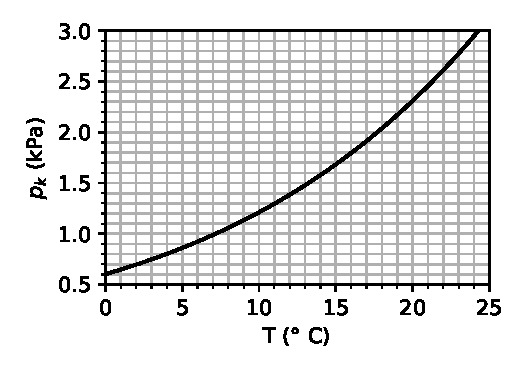
\includegraphics[width=0.5\textwidth]{2018-v3g-05-kullastunud-aur}
\par\end{center} 
\end{wrapfigure}
The insulation of a wall consists of an inner (of thermal conductivity $k_{1}=\SI{0.07}{W/\left(m\cdot K\right)}$) and an outer layer (that has a thermal conductivity $k_{2}=\SI{0.05}{W/\left(m\cdot K\right)}$). Between those layers there is a film layer to hinder the air’s movement through the wall. What condition does the width $L_{1},$ of the inner thermal insulation layer have to satisfy to avoid the condensation of water vapor in the wall? The width of the wall $L=L_{1}+L_{2}=\SI{30}{cm}$, $L_{2}$ is the width of the outer thermal insulation layer, the room temperature is $T_{1}=\SI{20}{\degreeCelsius}$, the relative humidity in the room is $\eta_{1}=\SI{60}{\percent}$ and the outside temperature $T_{2}=\SI{-20}{\degreeCelsius}$. The relation between the saturated vapor pressure of water and the temperature is shown in the figure.\\
\emph{Note.} Assume that the temperature in the insulation layer changes linearly with distance and the speed of the change is inversely proportional to thermal conductivity.

\hinteng
To avoid condensation on the film between the thermal insulation layers the temperature at the film must not fall beneath dew point. The dew point can be found from the graph by first finding the partial pressure of water vapor at room temperature and then finding its corresponding dew point.

\solueng
The film between the thermal insulation layers hinders the spreading of moist air. To avoid condensation the temperature in the film’s location must not fall below the dew point.\\
We can find the dew point from the graph by first finding the partial pressure of the water vapor at room temperature, calculating from it $\eta_{1}=\SI{60}{\percent}$ and then finding the dew point $T_{k}=\SI{12.0}{\degreeCelsius}.$ corresponding to it.
\begin{center}
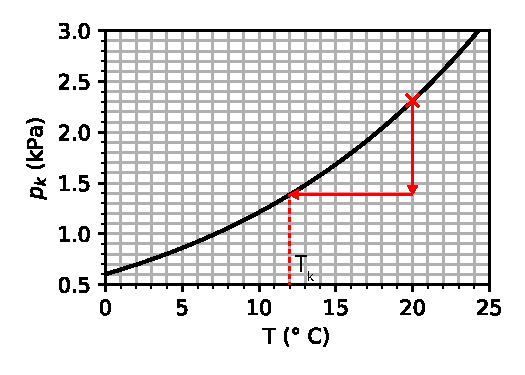
\includegraphics[scale=0.9]{2018-v3g-05-kullastunud-aur-lah}
\par\end{center}
Next we need to find the expression for the temperature at the film’s location ($T$). Assuming that the temperature in the thermal insulation layer changes linearly with the distance and the speed of change is inversely proportional to the thermal conductivity we can write down two equations when moving from inside to outside:
\begin{equation*}
\begin{cases}
\begin{array}{c}
T=T_{1}-\frac{\alpha}{k_{1}}L_{1}\\
T_{2}=T-\frac{\alpha}{k_{2}}L_{2},
\end{array}
\end{cases}
\end{equation*}
where $\alpha$ is an unknown proportionality factor. Solving these equations we get
\begin{equation*}
T=\frac{k_{2}T_{2}L_{1}+k_{1}T_{1}L_{2}}{k_{2}L_{1}+k_{1}L_{2}}.
\end{equation*}
And for final result we need to find the width $L_{1}$ of the inner thermal insulation layer at the limit case when the film’s temperature is equal to the dew point
\begin{equation*}
L_{1}=L\frac{k_{1}\left(T_{1}-T_{k}\right)}{k_{1}T_{1}-k_{2}T_{2}-\left(k_{1}-k_{2}\right)T_{k}}\approx\SI{7.8}{cm}
\end{equation*}
and to avoid condensation the width of the inner thermal insulation layer has to be smaller from that.
\probend